\documentclass[1p]{elsarticle_modified}
%\bibliographystyle{elsarticle-num}

%\usepackage[colorlinks]{hyperref}
%\usepackage{abbrmath_seonhwa} %\Abb, \Ascr, \Acal ,\Abf, \Afrak
\usepackage{amsfonts}
\usepackage{amssymb}
\usepackage{amsmath}
\usepackage{amsthm}
\usepackage{scalefnt}
\usepackage{amsbsy}
\usepackage{kotex}
\usepackage{caption}
\usepackage{subfig}
\usepackage{color}
\usepackage{graphicx}
\usepackage{xcolor} %% white, black, red, green, blue, cyan, magenta, yellow
\usepackage{float}
\usepackage{setspace}
\usepackage{hyperref}

\usepackage{tikz}
\usetikzlibrary{arrows}

\usepackage{multirow}
\usepackage{array} % fixed length table
\usepackage{hhline}

%%%%%%%%%%%%%%%%%%%%%
\makeatletter
\renewcommand*\env@matrix[1][\arraystretch]{%
	\edef\arraystretch{#1}%
	\hskip -\arraycolsep
	\let\@ifnextchar\new@ifnextchar
	\array{*\c@MaxMatrixCols c}}
\makeatother %https://tex.stackexchange.com/questions/14071/how-can-i-increase-the-line-spacing-in-a-matrix
%%%%%%%%%%%%%%%

\usepackage[normalem]{ulem}

\newcommand{\msout}[1]{\ifmmode\text{\sout{\ensuremath{#1}}}\else\sout{#1}\fi}
%SOURCE: \msout is \stkout macro in https://tex.stackexchange.com/questions/20609/strikeout-in-math-mode

\newcommand{\cancel}[1]{
	\ifmmode
	{\color{red}\msout{#1}}
	\else
	{\color{red}\sout{#1}}
	\fi
}

\newcommand{\add}[1]{
	{\color{blue}\uwave{#1}}
}

\newcommand{\replace}[2]{
	\ifmmode
	{\color{red}\msout{#1}}{\color{blue}\uwave{#2}}
	\else
	{\color{red}\sout{#1}}{\color{blue}\uwave{#2}}
	\fi
}

\newcommand{\Sol}{\mathcal{S}} %segment
\newcommand{\D}{D} %diagram
\newcommand{\A}{\mathcal{A}} %arc


%%%%%%%%%%%%%%%%%%%%%%%%%%%%%5 test

\def\sl{\operatorname{\textup{SL}}(2,\Cbb)}
\def\psl{\operatorname{\textup{PSL}}(2,\Cbb)}
\def\quan{\mkern 1mu \triangleright \mkern 1mu}

\theoremstyle{definition}
\newtheorem{thm}{Theorem}[section]
\newtheorem{prop}[thm]{Proposition}
\newtheorem{lem}[thm]{Lemma}
\newtheorem{ques}[thm]{Question}
\newtheorem{cor}[thm]{Corollary}
\newtheorem{defn}[thm]{Definition}
\newtheorem{exam}[thm]{Example}
\newtheorem{rmk}[thm]{Remark}
\newtheorem{alg}[thm]{Algorithm}

\newcommand{\I}{\sqrt{-1}}
\begin{document}

%\begin{frontmatter}
%
%\title{Boundary parabolic representations of knots up to 8 crossings}
%
%%% Group authors per affiliation:
%\author{Yunhi Cho} 
%\address{Department of Mathematics, University of Seoul, Seoul, Korea}
%\ead{yhcho@uos.ac.kr}
%
%
%\author{Seonhwa Kim} %\fnref{s_kim}}
%\address{Center for Geometry and Physics, Institute for Basic Science, Pohang, 37673, Korea}
%\ead{ryeona17@ibs.re.kr}
%
%\author{Hyuk Kim}
%\address{Department of Mathematical Sciences, Seoul National University, Seoul 08826, Korea}
%\ead{hyukkim@snu.ac.kr}
%
%\author{Seokbeom Yoon}
%\address{Department of Mathematical Sciences, Seoul National University, Seoul, 08826,  Korea}
%\ead{sbyoon15@snu.ac.kr}
%
%\begin{abstract}
%We find all boundary parabolic representation of knots up to 8 crossings.
%
%\end{abstract}
%\begin{keyword}
%    \MSC[2010] 57M25 
%\end{keyword}
%
%\end{frontmatter}

%\linenumbers
%\tableofcontents
%
\newcommand\colored[1]{\textcolor{white}{\rule[-0.35ex]{0.8em}{1.4ex}}\kern-0.8em\color{red} #1}%
%\newcommand\colored[1]{\textcolor{white}{ #1}\kern-2.17ex	\textcolor{white}{ #1}\kern-1.81ex	\textcolor{white}{ #1}\kern-2.15ex\color{red}#1	}

{\Large $\underline{11a_{185}~(K11a_{185})}$}

\setlength{\tabcolsep}{10pt}
\renewcommand{\arraystretch}{1.6}
\vspace{1cm}\begin{tabular}{m{100pt}>{\centering\arraybackslash}m{274pt}}
\multirow{5}{120pt}{
	\centering
	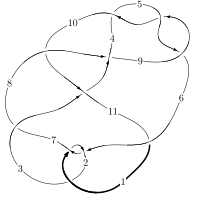
\includegraphics[width=112pt]{../../../GIT/diagram.site/Diagrams/png/434_11a_185.png}\\
\ \ \ A knot diagram\footnotemark}&
\allowdisplaybreaks
\textbf{Linearized knot diagam} \\
\cline{2-2}
 &
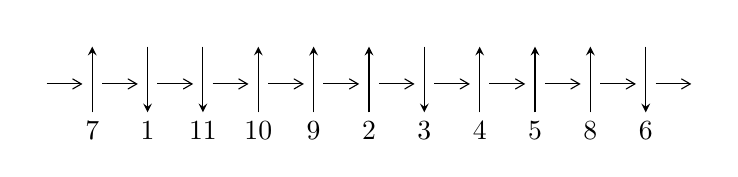
\begin{tikzpicture}[x=20pt, y=17pt]
	% nodes
	\node (C0) at (0, 0) {};
	\node (C1) at (1, 0) {};
	\node (C1U) at (1, +1) {};
	\node (C1D) at (1, -1) {7};

	\node (C2) at (2, 0) {};
	\node (C2U) at (2, +1) {};
	\node (C2D) at (2, -1) {1};

	\node (C3) at (3, 0) {};
	\node (C3U) at (3, +1) {};
	\node (C3D) at (3, -1) {11};

	\node (C4) at (4, 0) {};
	\node (C4U) at (4, +1) {};
	\node (C4D) at (4, -1) {10};

	\node (C5) at (5, 0) {};
	\node (C5U) at (5, +1) {};
	\node (C5D) at (5, -1) {9};

	\node (C6) at (6, 0) {};
	\node (C6U) at (6, +1) {};
	\node (C6D) at (6, -1) {2};

	\node (C7) at (7, 0) {};
	\node (C7U) at (7, +1) {};
	\node (C7D) at (7, -1) {3};

	\node (C8) at (8, 0) {};
	\node (C8U) at (8, +1) {};
	\node (C8D) at (8, -1) {4};

	\node (C9) at (9, 0) {};
	\node (C9U) at (9, +1) {};
	\node (C9D) at (9, -1) {5};

	\node (C10) at (10, 0) {};
	\node (C10U) at (10, +1) {};
	\node (C10D) at (10, -1) {8};

	\node (C11) at (11, 0) {};
	\node (C11U) at (11, +1) {};
	\node (C11D) at (11, -1) {6};
	\node (C12) at (12, 0) {};

	% arrows
	\draw[->,>={angle 60}]
	(C0) edge (C1) (C1) edge (C2) (C2) edge (C3) (C3) edge (C4) (C4) edge (C5) (C5) edge (C6) (C6) edge (C7) (C7) edge (C8) (C8) edge (C9) (C9) edge (C10) (C10) edge (C11) (C11) edge (C12) ;	\draw[->,>=stealth]
	(C1D) edge (C1U) (C2U) edge (C2D) (C3U) edge (C3D) (C4D) edge (C4U) (C5D) edge (C5U) (C6D) edge (C6U) (C7U) edge (C7D) (C8D) edge (C8U) (C9D) edge (C9U) (C10D) edge (C10U) (C11U) edge (C11D) ;
	\end{tikzpicture} \\
\hhline{~~} \\& 
\textbf{Solving Sequence} \\ \cline{2-2} 
 &
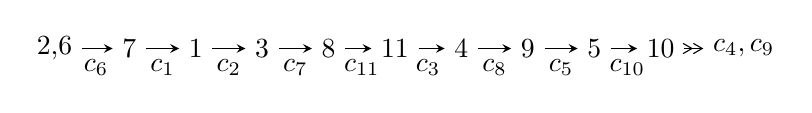
\begin{tikzpicture}[x=24pt, y=7pt]
	% node
	\node (A0) at (-1/8, 0) {2,6};
	\node (A1) at (1, 0) {7};
	\node (A2) at (2, 0) {1};
	\node (A3) at (3, 0) {3};
	\node (A4) at (4, 0) {8};
	\node (A5) at (5, 0) {11};
	\node (A6) at (6, 0) {4};
	\node (A7) at (7, 0) {9};
	\node (A8) at (8, 0) {5};
	\node (A9) at (9, 0) {10};
	\node (C1) at (1/2, -1) {$c_{6}$};
	\node (C2) at (3/2, -1) {$c_{1}$};
	\node (C3) at (5/2, -1) {$c_{2}$};
	\node (C4) at (7/2, -1) {$c_{7}$};
	\node (C5) at (9/2, -1) {$c_{11}$};
	\node (C6) at (11/2, -1) {$c_{3}$};
	\node (C7) at (13/2, -1) {$c_{8}$};
	\node (C8) at (15/2, -1) {$c_{5}$};
	\node (C9) at (17/2, -1) {$c_{10}$};
	\node (A10) at (41/4, 0) {$c_{4},c_{9}$};

	% edge
	\draw[->,>=stealth]	
	(A0) edge (A1) (A1) edge (A2) (A2) edge (A3) (A3) edge (A4) (A4) edge (A5) (A5) edge (A6) (A6) edge (A7) (A7) edge (A8) (A8) edge (A9) ;
	\draw[->>,>={angle 60}]	
	(A9) edge (A10);
\end{tikzpicture} \\ 

\end{tabular} \\

\footnotetext{
The image of knot diagram is generated by the software ``\textbf{Draw programme}" developed by Andrew Bartholomew(\url{http://www.layer8.co.uk/maths/draw/index.htm\#Running-draw}), where we modified some parts for our purpose(\url{https://github.com/CATsTAILs/LinksPainter}).
}\phantom \\ \newline 
\centering \textbf{Ideals for irreducible components\footnotemark of $X_{\text{par}}$} 
 
\begin{align*}
I^u_{1}&=\langle 
u^{54}+u^{53}+\cdots+u+1\rangle \\
\\
\end{align*}
\raggedright * 1 irreducible components of $\dim_{\mathbb{C}}=0$, with total 54 representations.\\
\footnotetext{All coefficients of polynomials are rational numbers. But the coefficients are sometimes approximated in decimal forms when there is not enough margin.}
\newpage
\renewcommand{\arraystretch}{1}
\centering \section*{I. $I^u_{1}= \langle u^{54}+u^{53}+\cdots+u+1 \rangle$}
\flushleft \textbf{(i) Arc colorings}\\
\begin{tabular}{m{7pt} m{180pt} m{7pt} m{180pt} }
\flushright $a_{2}=$&$\begin{pmatrix}0\\u\end{pmatrix}$ \\
\flushright $a_{6}=$&$\begin{pmatrix}1\\0\end{pmatrix}$ \\
\flushright $a_{7}=$&$\begin{pmatrix}1\\- u^2\end{pmatrix}$ \\
\flushright $a_{1}=$&$\begin{pmatrix}- u\\u^3+u\end{pmatrix}$ \\
\flushright $a_{3}=$&$\begin{pmatrix}- u^3\\u^5+u^3+u\end{pmatrix}$ \\
\flushright $a_{8}=$&$\begin{pmatrix}- u^6- u^4+1\\u^8+2 u^6+2 u^4\end{pmatrix}$ \\
\flushright $a_{11}=$&$\begin{pmatrix}u^3\\u^3+u\end{pmatrix}$ \\
\flushright $a_{4}=$&$\begin{pmatrix}- u^{11}-2 u^9-2 u^7- u^3\\- u^{11}-3 u^9-4 u^7- u^5+u^3+u\end{pmatrix}$ \\
\flushright $a_{9}=$&$\begin{pmatrix}u^{30}+7 u^{28}+\cdots-2 u^{12}+1\\u^{30}+8 u^{28}+\cdots+4 u^6- u^2\end{pmatrix}$ \\
\flushright $a_{5}=$&$\begin{pmatrix}- u^{47}-12 u^{45}+\cdots-20 u^9-8 u^7\\u^{49}+13 u^{47}+\cdots-2 u^5+u\end{pmatrix}$ \\
\flushright $a_{10}=$&$\begin{pmatrix}- u^{17}-4 u^{15}-7 u^{13}-4 u^{11}+3 u^9+6 u^7+2 u^5- u\\u^{19}+5 u^{17}+12 u^{15}+15 u^{13}+9 u^{11}- u^9-4 u^7-2 u^5+u^3+u\end{pmatrix}$\\ \flushright $a_{10}=$&$\begin{pmatrix}- u^{17}-4 u^{15}-7 u^{13}-4 u^{11}+3 u^9+6 u^7+2 u^5- u\\u^{19}+5 u^{17}+12 u^{15}+15 u^{13}+9 u^{11}- u^9-4 u^7-2 u^5+u^3+u\end{pmatrix}$\\&\end{tabular}
\flushleft \textbf{(ii) Obstruction class $= -1$}\\~\\
\flushleft \textbf{(iii) Cusp Shapes $= -4 u^{52}-4 u^{51}+\cdots+4 u^2-2$}\\~\\
\newpage\renewcommand{\arraystretch}{1}
\flushleft \textbf{(iv) u-Polynomials at the component}\newline \\
\begin{tabular}{m{50pt}|m{274pt}}
Crossings & \hspace{64pt}u-Polynomials at each crossing \\
\hline $$\begin{aligned}c_{1},c_{6}\end{aligned}$$&$\begin{aligned}
&u^{54}+u^{53}+\cdots+u+1
\end{aligned}$\\
\hline $$\begin{aligned}c_{2}\end{aligned}$$&$\begin{aligned}
&u^{54}+29 u^{53}+\cdots- u+1
\end{aligned}$\\
\hline $$\begin{aligned}c_{3}\end{aligned}$$&$\begin{aligned}
&u^{54}-7 u^{53}+\cdots-47 u+5
\end{aligned}$\\
\hline $$\begin{aligned}c_{4},c_{5},c_{9}\end{aligned}$$&$\begin{aligned}
&u^{54}- u^{53}+\cdots- u+1
\end{aligned}$\\
\hline $$\begin{aligned}c_{7},c_{11}\end{aligned}$$&$\begin{aligned}
&u^{54}- u^{53}+\cdots+u+1
\end{aligned}$\\
\hline $$\begin{aligned}c_{8}\end{aligned}$$&$\begin{aligned}
&u^{54}+u^{53}+\cdots+11 u+1
\end{aligned}$\\
\hline $$\begin{aligned}c_{10}\end{aligned}$$&$\begin{aligned}
&u^{54}+11 u^{53}+\cdots+1951 u+187
\end{aligned}$\\
\hline
\end{tabular}\\~\\
\newpage\renewcommand{\arraystretch}{1}
\flushleft \textbf{(v) Riley Polynomials at the component}\newline \\
\begin{tabular}{m{50pt}|m{274pt}}
Crossings & \hspace{64pt}Riley Polynomials at each crossing \\
\hline $$\begin{aligned}c_{1},c_{6}\end{aligned}$$&$\begin{aligned}
&y^{54}+29 y^{53}+\cdots- y+1
\end{aligned}$\\
\hline $$\begin{aligned}c_{2}\end{aligned}$$&$\begin{aligned}
&y^{54}-7 y^{53}+\cdots-5 y+1
\end{aligned}$\\
\hline $$\begin{aligned}c_{3}\end{aligned}$$&$\begin{aligned}
&y^{54}-3 y^{53}+\cdots+631 y+25
\end{aligned}$\\
\hline $$\begin{aligned}c_{4},c_{5},c_{9}\end{aligned}$$&$\begin{aligned}
&y^{54}+49 y^{53}+\cdots- y+1
\end{aligned}$\\
\hline $$\begin{aligned}c_{7},c_{11}\end{aligned}$$&$\begin{aligned}
&y^{54}-43 y^{53}+\cdots-97 y+1
\end{aligned}$\\
\hline $$\begin{aligned}c_{8}\end{aligned}$$&$\begin{aligned}
&y^{54}+5 y^{53}+\cdots-49 y+1
\end{aligned}$\\
\hline $$\begin{aligned}c_{10}\end{aligned}$$&$\begin{aligned}
&y^{54}+21 y^{53}+\cdots+184179 y+34969
\end{aligned}$\\
\hline
\end{tabular}\\~\\
\newpage\flushleft \textbf{(vi) Complex Volumes and Cusp Shapes}
$$\begin{array}{c|c|c}  
\text{Solutions to }I^u_{1}& \I (\text{vol} + \sqrt{-1}CS) & \text{Cusp shape}\\
 \hline 
\begin{aligned}
u &= -0.526458 + 0.850149 I\end{aligned}
 & \phantom{-}1.84506 - 5.20730 I & \phantom{-}6.07211 + 8.44255 I \\ \hline\begin{aligned}
u &= -0.526458 - 0.850149 I\end{aligned}
 & \phantom{-}1.84506 + 5.20730 I & \phantom{-}6.07211 - 8.44255 I \\ \hline\begin{aligned}
u &= \phantom{-}0.063963 + 0.969473 I\end{aligned}
 & -2.01199 + 1.57241 I & -2.93647 - 4.70910 I \\ \hline\begin{aligned}
u &= \phantom{-}0.063963 - 0.969473 I\end{aligned}
 & -2.01199 - 1.57241 I & -2.93647 + 4.70910 I \\ \hline\begin{aligned}
u &= \phantom{-}0.542026 + 0.876210 I\end{aligned}
 & -3.38874 + 8.60756 I & \phantom{-}0.88746 - 8.62489 I \\ \hline\begin{aligned}
u &= \phantom{-}0.542026 - 0.876210 I\end{aligned}
 & -3.38874 - 8.60756 I & \phantom{-}0.88746 + 8.62489 I \\ \hline\begin{aligned}
u &= -0.068795 + 1.043570 I\end{aligned}
 & -7.55344 - 4.33327 I & -6.71453 + 3.78697 I \\ \hline\begin{aligned}
u &= -0.068795 - 1.043570 I\end{aligned}
 & -7.55344 + 4.33327 I & -6.71453 - 3.78697 I \\ \hline\begin{aligned}
u &= -0.404606 + 0.965250 I\end{aligned}
 & -5.19453 - 0.85164 I & -2.69916 + 2.79194 I \\ \hline\begin{aligned}
u &= -0.404606 - 0.965250 I\end{aligned}
 & -5.19453 + 0.85164 I & -2.69916 - 2.79194 I \\ \hline\begin{aligned}
u &= \phantom{-}0.459955 + 0.798537 I\end{aligned}
 & \phantom{-}0.23556 + 1.92632 I & \phantom{-}2.54464 - 3.58852 I \\ \hline\begin{aligned}
u &= \phantom{-}0.459955 - 0.798537 I\end{aligned}
 & \phantom{-}0.23556 - 1.92632 I & \phantom{-}2.54464 + 3.58852 I \\ \hline\begin{aligned}
u &= \phantom{-}0.514528 + 0.758613 I\end{aligned}
 & \phantom{-}0.15792 + 2.10554 I & \phantom{-}4.75076 - 4.16265 I \\ \hline\begin{aligned}
u &= \phantom{-}0.514528 - 0.758613 I\end{aligned}
 & \phantom{-}0.15792 - 2.10554 I & \phantom{-}4.75076 + 4.16265 I \\ \hline\begin{aligned}
u &= -0.521169 + 0.661679 I\end{aligned}
 & \phantom{-}2.37968 + 0.93113 I & \phantom{-}8.32580 - 1.37232 I \\ \hline\begin{aligned}
u &= -0.521169 - 0.661679 I\end{aligned}
 & \phantom{-}2.37968 - 0.93113 I & \phantom{-}8.32580 + 1.37232 I \\ \hline\begin{aligned}
u &= \phantom{-}0.555404 + 0.618983 I\end{aligned}
 & -2.66786 - 4.19841 I & \phantom{-}2.85328 + 2.26313 I \\ \hline\begin{aligned}
u &= \phantom{-}0.555404 - 0.618983 I\end{aligned}
 & -2.66786 + 4.19841 I & \phantom{-}2.85328 - 2.26313 I \\ \hline\begin{aligned}
u &= -0.812471 + 0.137850 I\end{aligned}
 & -6.92259 + 9.00910 I & -0.82614 - 5.72677 I \\ \hline\begin{aligned}
u &= -0.812471 - 0.137850 I\end{aligned}
 & -6.92259 - 9.00910 I & -0.82614 + 5.72677 I \\ \hline\begin{aligned}
u &= -0.409939 + 1.110810 I\end{aligned}
 & -5.37080 - 0.77260 I & \phantom{-0.000000 } 0 \\ \hline\begin{aligned}
u &= -0.409939 - 1.110810 I\end{aligned}
 & -5.37080 + 0.77260 I & \phantom{-0.000000 } 0 \\ \hline\begin{aligned}
u &= \phantom{-}0.803336 + 0.074667 I\end{aligned}
 & -8.69949 + 0.21899 I & -3.12382 - 0.07866 I \\ \hline\begin{aligned}
u &= \phantom{-}0.803336 - 0.074667 I\end{aligned}
 & -8.69949 - 0.21899 I & -3.12382 + 0.07866 I \\ \hline\begin{aligned}
u &= \phantom{-}0.793006 + 0.135744 I\end{aligned}
 & -1.35714 - 5.52569 I & \phantom{-}3.45218 + 5.82582 I \\ \hline\begin{aligned}
u &= \phantom{-}0.793006 - 0.135744 I\end{aligned}
 & -1.35714 + 5.52569 I & \phantom{-}3.45218 - 5.82582 I \\ \hline\begin{aligned}
u &= \phantom{-}0.465718 + 1.132140 I\end{aligned}
 & -1.40488 + 3.87836 I & \phantom{-0.000000 } 0 \\ \hline\begin{aligned}
u &= \phantom{-}0.465718 - 1.132140 I\end{aligned}
 & -1.40488 - 3.87836 I & \phantom{-0.000000 } 0 \\ \hline\begin{aligned}
u &= -0.768273 + 0.105402 I\end{aligned}
 & -2.42732 + 1.73641 I & \phantom{-}0.699777 + 0.008860 I \\ \hline\begin{aligned}
u &= -0.768273 - 0.105402 I\end{aligned}
 & -2.42732 - 1.73641 I & \phantom{-}0.699777 - 0.008860 I\\
 \hline 
 \end{array}$$\newpage$$\begin{array}{c|c|c}  
\text{Solutions to }I^u_{1}& \I (\text{vol} + \sqrt{-1}CS) & \text{Cusp shape}\\
 \hline 
\begin{aligned}
u &= -0.492150 + 1.152340 I\end{aligned}
 & -4.72150 - 7.14315 I & \phantom{-0.000000 } 0 \\ \hline\begin{aligned}
u &= -0.492150 - 1.152340 I\end{aligned}
 & -4.72150 + 7.14315 I & \phantom{-0.000000 } 0 \\ \hline\begin{aligned}
u &= -0.403427 + 1.196670 I\end{aligned}
 & -6.22025 - 2.29095 I & \phantom{-0.000000 } 0 \\ \hline\begin{aligned}
u &= -0.403427 - 1.196670 I\end{aligned}
 & -6.22025 + 2.29095 I & \phantom{-0.000000 } 0 \\ \hline\begin{aligned}
u &= \phantom{-}0.382721 + 1.204180 I\end{aligned}
 & -5.34368 - 1.56137 I & \phantom{-0.000000 } 0 \\ \hline\begin{aligned}
u &= \phantom{-}0.382721 - 1.204180 I\end{aligned}
 & -5.34368 + 1.56137 I & \phantom{-0.000000 } 0 \\ \hline\begin{aligned}
u &= -0.378306 + 1.216650 I\end{aligned}
 & -11.00630 + 4.98743 I & \phantom{-0.000000 } 0 \\ \hline\begin{aligned}
u &= -0.378306 - 1.216650 I\end{aligned}
 & -11.00630 - 4.98743 I & \phantom{-0.000000 } 0 \\ \hline\begin{aligned}
u &= \phantom{-}0.415619 + 1.215680 I\end{aligned}
 & -12.53210 + 4.46314 I & \phantom{-0.000000 } 0 \\ \hline\begin{aligned}
u &= \phantom{-}0.415619 - 1.215680 I\end{aligned}
 & -12.53210 - 4.46314 I & \phantom{-0.000000 } 0 \\ \hline\begin{aligned}
u &= -0.494467 + 1.187320 I\end{aligned}
 & -5.57287 - 6.38943 I & \phantom{-0.000000 } 0 \\ \hline\begin{aligned}
u &= -0.494467 - 1.187320 I\end{aligned}
 & -5.57287 + 6.38943 I & \phantom{-0.000000 } 0 \\ \hline\begin{aligned}
u &= -0.688011 + 0.172752 I\end{aligned}
 & -1.90661 + 2.65629 I & \phantom{-}2.99397 - 3.57576 I \\ \hline\begin{aligned}
u &= -0.688011 - 0.172752 I\end{aligned}
 & -1.90661 - 2.65629 I & \phantom{-}2.99397 + 3.57576 I \\ \hline\begin{aligned}
u &= \phantom{-}0.508429 + 1.190650 I\end{aligned}
 & -4.45647 + 10.31740 I & \phantom{-0.000000 } 0 \\ \hline\begin{aligned}
u &= \phantom{-}0.508429 - 1.190650 I\end{aligned}
 & -4.45647 - 10.31740 I & \phantom{-0.000000 } 0 \\ \hline\begin{aligned}
u &= \phantom{-}0.486868 + 1.204310 I\end{aligned}
 & -12.02490 + 4.47153 I & \phantom{-0.000000 } 0 \\ \hline\begin{aligned}
u &= \phantom{-}0.486868 - 1.204310 I\end{aligned}
 & -12.02490 - 4.47153 I & \phantom{-0.000000 } 0 \\ \hline\begin{aligned}
u &= -0.513281 + 1.197090 I\end{aligned}
 & -10.0524 - 13.8722 I & \phantom{-0.000000 } 0 \\ \hline\begin{aligned}
u &= -0.513281 - 1.197090 I\end{aligned}
 & -10.0524 + 13.8722 I & \phantom{-0.000000 } 0 \\ \hline\begin{aligned}
u &= -0.553091 + 0.375407 I\end{aligned}
 & -3.44062 - 3.02821 I & \phantom{-}2.33743 + 2.90410 I \\ \hline\begin{aligned}
u &= -0.553091 - 0.375407 I\end{aligned}
 & -3.44062 + 3.02821 I & \phantom{-}2.33743 - 2.90410 I \\ \hline\begin{aligned}
u &= \phantom{-}0.542871 + 0.222612 I\end{aligned}
 & \phantom{-}1.223040 + 0.207996 I & \phantom{-}8.65252 - 1.10768 I \\ \hline\begin{aligned}
u &= \phantom{-}0.542871 - 0.222612 I\end{aligned}
 & \phantom{-}1.223040 - 0.207996 I & \phantom{-}8.65252 + 1.10768 I\\
 \hline 
 \end{array}$$\newpage
\newpage\renewcommand{\arraystretch}{1}
\centering \section*{ II. u-Polynomials}
\begin{tabular}{m{50pt}|m{274pt}}
Crossings & \hspace{64pt}u-Polynomials at each crossing \\
\hline $$\begin{aligned}c_{1},c_{6}\end{aligned}$$&$\begin{aligned}
&u^{54}+u^{53}+\cdots+u+1
\end{aligned}$\\
\hline $$\begin{aligned}c_{2}\end{aligned}$$&$\begin{aligned}
&u^{54}+29 u^{53}+\cdots- u+1
\end{aligned}$\\
\hline $$\begin{aligned}c_{3}\end{aligned}$$&$\begin{aligned}
&u^{54}-7 u^{53}+\cdots-47 u+5
\end{aligned}$\\
\hline $$\begin{aligned}c_{4},c_{5},c_{9}\end{aligned}$$&$\begin{aligned}
&u^{54}- u^{53}+\cdots- u+1
\end{aligned}$\\
\hline $$\begin{aligned}c_{7},c_{11}\end{aligned}$$&$\begin{aligned}
&u^{54}- u^{53}+\cdots+u+1
\end{aligned}$\\
\hline $$\begin{aligned}c_{8}\end{aligned}$$&$\begin{aligned}
&u^{54}+u^{53}+\cdots+11 u+1
\end{aligned}$\\
\hline $$\begin{aligned}c_{10}\end{aligned}$$&$\begin{aligned}
&u^{54}+11 u^{53}+\cdots+1951 u+187
\end{aligned}$\\
\hline
\end{tabular}\newpage\renewcommand{\arraystretch}{1}
\centering \section*{ III. Riley Polynomials}
\begin{tabular}{m{50pt}|m{274pt}}
Crossings & \hspace{64pt}Riley Polynomials at each crossing \\
\hline $$\begin{aligned}c_{1},c_{6}\end{aligned}$$&$\begin{aligned}
&y^{54}+29 y^{53}+\cdots- y+1
\end{aligned}$\\
\hline $$\begin{aligned}c_{2}\end{aligned}$$&$\begin{aligned}
&y^{54}-7 y^{53}+\cdots-5 y+1
\end{aligned}$\\
\hline $$\begin{aligned}c_{3}\end{aligned}$$&$\begin{aligned}
&y^{54}-3 y^{53}+\cdots+631 y+25
\end{aligned}$\\
\hline $$\begin{aligned}c_{4},c_{5},c_{9}\end{aligned}$$&$\begin{aligned}
&y^{54}+49 y^{53}+\cdots- y+1
\end{aligned}$\\
\hline $$\begin{aligned}c_{7},c_{11}\end{aligned}$$&$\begin{aligned}
&y^{54}-43 y^{53}+\cdots-97 y+1
\end{aligned}$\\
\hline $$\begin{aligned}c_{8}\end{aligned}$$&$\begin{aligned}
&y^{54}+5 y^{53}+\cdots-49 y+1
\end{aligned}$\\
\hline $$\begin{aligned}c_{10}\end{aligned}$$&$\begin{aligned}
&y^{54}+21 y^{53}+\cdots+184179 y+34969
\end{aligned}$\\
\hline
\end{tabular}
\vskip 2pc
\end{document}